\documentclass[a4paper,12pt]{ctexart}
\usepackage{geometry}
\geometry{left=2.0cm, right=2.0cm, top=2.5cm, bottom=2.5cm}
\usepackage{amsmath, amssymb, amstext}
\usepackage{graphicx}
\usepackage{xcolor}
\usepackage{float}
\usepackage{tikz}
\usepackage{pgfplots}
\usepackage{enumitem}
\usepackage{cases}
\usepackage{tcolorbox}
\usetikzlibrary{arrows.meta, positioning, patterns}
\pgfplotsset{compat=1.18}
\linespread{1.5}

% Colors
\definecolor{myorange}{RGB}{235, 120, 50}
\definecolor{myblue}{RGB}{0, 114, 189}
\definecolor{highlightred}{RGB}{200, 30, 30}
\definecolor{notepurple}{RGB}{230, 230, 250}
\definecolor{boxpurple}{RGB}{128, 0, 128}

% Environments
\newenvironment{purplebox}
  {\begin{tcolorbox}[colback=white, colframe=boxpurple, boxrule=1pt, sharp corners, title=\textbf{定义/定理/核心公式}]}
  {\end{tcolorbox}}

\newenvironment{rednote}
  {\begin{tcolorbox}[colback=notepurple, colframe=highlightred, boxrule=1pt, title=\textbf{重点/技巧/手写笔记}]}
  {\end{tcolorbox}}

\newenvironment{greenbox}
  {\begin{tcolorbox}[colback=white, colframe=green!60!black, boxrule=1pt, sharp corners]}
  {\end{tcolorbox}}

\newcommand{\zh}[1]{\par\smallskip\noindent\textbf{#1}\par\smallskip}

\title{\textbf{考研数学 - 高数总结 (全)}}
\author{fifine}
\date{\today}

\begin{document}

\maketitle
\tableofcontents
\newpage

% ====================================
% Content from 0.tex
% ====================================
\section*{初等数学公式}

\subsection*{常见的三角函数图像}

\begin{figure}[H]
    \centering
    \begin{minipage}{0.48\textwidth}
        \centering
        \begin{tikzpicture}[scale=0.7]
            \begin{axis}[
                axis lines=middle,
                xmin=-4.9, xmax=4.9,
                ymin=-3.5, ymax=3.5,
                xtick={-4.71, -3.14, -1.57, 1.57, 3.14, 4.71},
                % 修复：去掉了奇怪的 \\end{cases} 乱码
                xticklabels={$\frac{3\pi}{2}$, $\pi$, $\frac{\pi}{2}$, $\frac{\pi}{2}$, $\pi$, $\frac{3\pi}{2}$},
                ytick={-1, 1, 2, 3},
                grid=both,
                major grid style={line width=.2pt,draw=gray!30},
                width=\linewidth,
                height=0.8\linewidth,
                tick label style={font=\tiny},
                clip=true
            ]
                % sin(x)
                \addplot[domain=-4.9:4.9, samples=100, color=myblue, thick] {sin(deg(x))};
                \node[color=myblue, font=\tiny] at (axis cs: 2.5, 0.8) {$\sin(x)$};
                
                % cos(x)
                \addplot[domain=-4.9:4.9, samples=100, color=highlightred, thick] {cos(deg(x))};
                \node[color=highlightred, font=\tiny] at (axis cs: 1.2, 0.8) {$\cos(x)$};
                
                % tan(x)
                \addplot[domain=-1.4:1.4, samples=50, color=myorange, thick] {tan(deg(x))};
                \addplot[domain=1.74:4.5, samples=50, color=myorange, thick] {tan(deg(x))};
                \addplot[domain=-4.5:-1.74, samples=50, color=myorange, thick] {tan(deg(x))};
                \node[color=myorange, font=\tiny] at (axis cs: -1.0, 2.5) {$\tan(x)$};
                
            \end{axis}
            \node[font=\scriptsize, below] at (current bounding box.south) {正弦、余弦以及正切函数};
        \end{tikzpicture}
    \end{minipage}
    \hfill
    \begin{minipage}{0.48\textwidth}
        \centering
        \begin{tikzpicture}[scale=0.7]
             \begin{axis}[
                axis lines=middle,
                xmin=-2.2, xmax=2.2,
                ymin=-1.8, ymax=3.5,
                xtick={-2, -1, 1, 2},
                ytick={-1.57, 1.57, 3.14},
                % 修复：去掉了奇怪的 \\end{cases} 乱码
                yticklabels={$-\frac{1}{2}\pi$, $\frac{1}{2}\pi$, $\pi$},
                grid=both,
                major grid style={line width=.2pt,draw=gray!30},
                width=\linewidth,
                height=0.8\linewidth,
                tick label style={font=\tiny}
            ]
                % arcsin
                \addplot[domain=-1:1, samples=100, color=myblue, thick] {rad(asin(x))};
                \node[color=myblue, font=\tiny, anchor=west] at (axis cs: 1.1, 1.0) {$\arcsin(x)$};
                
                % arccos
                \addplot[domain=-1:1, samples=100, color=highlightred, thick] {rad(acos(x))};
                \node[color=highlightred, font=\tiny, anchor=east] at (axis cs: -0.5, 2.8) {$\arccos(x)$};
                
                % arctan
                \addplot[domain=-2.2:2.2, samples=100, color=myorange, thick] {rad(atan(x))};
                \node[color=myorange, font=\tiny, anchor=west] at (axis cs: 1.1, 0.5) {$\arctan(x)$};
                
                \draw[dashed, gray] (axis cs:-2, 1.57) -- (axis cs:2, 1.57);
                \draw[dashed, gray] (axis cs:-2, -1.57) -- (axis cs:2, -1.57);
            \end{axis}
            \node[font=\scriptsize, below] at (current bounding box.south) {反正弦、反余弦以及反正切函数};
        \end{tikzpicture}
    \end{minipage}
\end{figure}

\subsection*{常见的三角函数公式}

\textbf{六角形法则}

\begin{figure}[H]
    \centering
    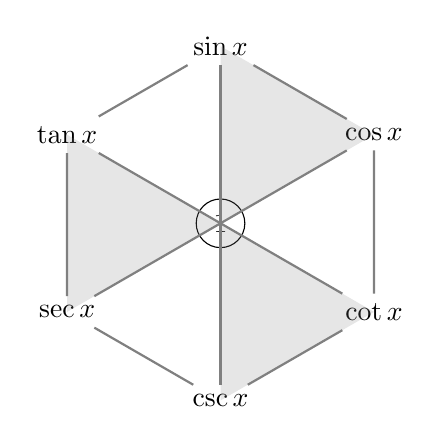
\begin{tikzpicture}[scale=1.5]
        % 修复：去掉了节点文字周围的 \\end{cases}
        % Hexagon vertices
        \node (sin) at (90:1.5) {$\sin x$};
        \node (cos) at (30:1.5) {$\cos x$};
        \node (cot) at (-30:1.5) {$\cot x$};
        \node (csc) at (-90:1.5) {$\csc x$};
        \node (sec) at (-150:1.5) {$\sec x$};
        \node (tan) at (150:1.5) {$\tan x$};
        \node[circle, draw, fill=white] (one) at (0,0) {1};

        % Edges
        \draw[thick, gray] (sin) -- (cos) -- (cot) -- (csc) -- (sec) -- (tan) -- (sin);
        
        % Diagonals
        \draw[thick, gray] (sin) -- (csc);
        \draw[thick, gray] (cos) -- (sec);
        \draw[thick, gray] (tan) -- (cot);
        
        % Shading
        \fill[gray, opacity=0.2] (0,0) -- (90:1.5) -- (30:1.5) -- cycle;
        \fill[gray, opacity=0.2] (0,0) -- (-30:1.5) -- (-90:1.5) -- cycle;
        \fill[gray, opacity=0.2] (0,0) -- (-150:1.5) -- (150:1.5) -- cycle;
    \end{tikzpicture}
\end{figure}


\section*{常用三角函数公式}

\[ \cos^2 x + \sin^2 x = 1 \quad \cos^2 x - \sin^2 x = \cos 2x \]

\[ 2\sin x \cos x = \sin 2x \]

\[ 1 - \cos 2x = 2\sin^2 x \quad 1 + \cos 2x = 2\cos^2 x \]

\[ 1 + \tan^2 x = \frac{1}{\cos^2 x} = \sec^2 x \quad 1 + \cot^2 x = \frac{1}{\sin^2 x} = \csc^2 x \]

\[ \sin x \sin y = -\frac{1}{2}[\cos(x+y) - \cos(x-y)] \]

\[ \cos x \cos y = \frac{1}{2}[\cos(x+y) + \cos(x-y)] \]

\[ \sin x \cos y = \frac{1}{2}[\sin(x+y) + \sin(x-y)] \]

\section*{和差化积公式}

\begin{align*}
    \sin \alpha + \sin \beta &= 2\sin\frac{\alpha+\beta}{2}\cos\frac{\alpha-\beta}{2} \\
    \sin \alpha - \sin \beta &= 2\cos\frac{\alpha+\beta}{2}\sin\frac{\alpha-\beta}{2} \\
    \cos \alpha + \cos \beta &= 2\cos\frac{\alpha+\beta}{2}\cos\frac{\alpha-\beta}{2} \\
    \cos \alpha - \cos \beta &= -2\sin\frac{\alpha+\beta}{2}\sin\frac{\alpha-\beta}{2}
\end{align*}
*(注：原文最后一个公式系数为 $2\sin...$，但标准公式应包含负号或调整顺序，此处依据原文截图看似有负号或书写习惯，标准为$-2\sin\sin$)*

\section*{倍角公式}

\begin{align*}
    \sin 2\alpha &= 2\sin \alpha \cos \alpha \\
    \cos 2\alpha &= 2\cos^2 \alpha - 1 = 1 - 2\sin^2 \alpha = \cos^2 \alpha - \sin^2 \alpha \\
    \cot 2\alpha &= \frac{\cot^2 \alpha - 1}{2\cot \alpha} \\
    \tan 2\alpha &= \frac{2\tan \alpha}{1 - \tan^2 \alpha}
\end{align*}

\begin{align*}
    \sin 3\alpha &= 3\sin \alpha - 4\sin^3 \alpha \\
    \cos 3\alpha &= 4\cos^3 \alpha - 3\cos \alpha \\
    \tan 3\alpha &= \frac{3\tan \alpha - \tan^3 \alpha}{1 - 3\tan^2 \alpha}
\end{align*}

\section*{三角形诱导公式}

\noindent\textbf{口诀：}奇变偶不变（对于 $n$ 而言），符号（对于 $x + n \cdot \frac{\pi}{2}$）看象限。
将$\sin(x + n \cdot \pi/2)$ 中的 $x$ 看作是锐角。

\vspace{0.5cm}
\noindent\textbf{手写笔记补充（反三角函数与三角函数嵌套及其他）：}

\begin{itemize}
    \item \textbf{补充公式：}
    \[ \arctan x + \arctan \frac{1}{x} = \begin{cases} \frac{\pi}{2}, & x > 0 \\ -\frac{\pi}{2}, & x < 0 \end{cases} \]
    
    \item \textbf{嵌套化简：}
    \[ \arcsin(\sin t) = \begin{cases} t, & t \in [0, \frac{\pi}{2}] \\ \pi - t, & t \in [\frac{\pi}{2}, \frac{3\pi}{2}] \end{cases} \]
    
    \item \textbf{六边形推论（倒数关系）：}
    \[ \csc x = \frac{1}{\sin x}, \quad \sec x = \frac{1}{\cos x}, \quad \cot x = \frac{1}{\tan x} \]
    \[ \tan x = \frac{\sin x}{\cos x}, \quad \cot x = \frac{\cos x}{\sin x} \]
    
    \item \textbf{平方关系：}
    \[ \sin^2 x + \cos^2 x = 1, \quad 1 + \tan^2 x = \sec^2 x, \quad 1 + \cot^2 x = \csc^2 x \]
    
    \item \textbf{诱导公式补充（配角公式）：}
    \[ \sin(x) = \cos(\frac{\pi}{2} - x) \]
    \[ \arctan x + \arctan \frac{1}{x} = \text{const} \]
    \[ \arcsin x + \arccos x = \frac{\pi}{2} \]
\end{itemize}

\section*{三角函数与三角函数周期计算}
\noindent \textbf{1. 基本周期公式}
\begin{itemize}
    \item $y = \sin(\omega x + \varphi)$ 和 $y = \cos(\omega x + \varphi)$ 的最小正周期为 $T = \frac{2\pi}{|\omega|}$。
    \item $y = \tan(\omega x + \varphi)$ 的最小正周期为 $T = \frac{\pi}{|\omega|}$。
    \item $y = |\sin(\omega x + \varphi)|$ 和 $y = |\cos(\omega x + \varphi)|$ 的最小正周期为 $T = \frac{\pi}{|\omega|}$。
\end{itemize}

\vspace{0.3cm}
\noindent \textbf{2. 周期函数的运算法则}
\begin{itemize}
    \item 若 $f(x)$ 的周期为 $T$，则 $f(\omega x)$ 的周期为 $\frac{T}{|\omega|}$。
    \item \textbf{最小公倍数法}：若 $y = f(x) + g(x)$，其中 $f(x)$ 周期为 $T_1$，$g(x)$ 周期为 $T_2$，且 $\frac{T_1}{T_2} \in \mathbb{Q}$，则和函数的周期 $T$ 为 $T_1, T_2$ 的最小公倍数。
\end{itemize}

\begin{rednote}
    \textbf{常见结论补充：}
    \begin{enumerate}
        \item $y = \sin^2 x$ 和 $y = \cos^2 x$ 的周期均为 $\pi$。（降幂后变 $\cos 2x$）
        \item $y = |\sin x| + |\cos x|$ 的周期为 $\frac{\pi}{2}$。
        \item $y = \sin x + \cos x$ 的周期为 $2\pi$。
    \end{enumerate}
\end{rednote}

\noindent \textbf{3. 抽象函数的周期性结论（重要）}
\begin{itemize}
    \item \textbf{利用函数关系式判断：}
    \begin{enumerate}
        \item $f(x+a) = -f(x) \Rightarrow T = 2a$。
        \item $f(x+a) = \frac{1}{f(x)}$ 或 $f(x+a) = -\frac{1}{f(x)} \Rightarrow T = 2a$。
        \item $f(x+a) + f(x) = C$ （$C$为常数） $\Rightarrow T = 2a$。
    \end{enumerate}
    \item \textbf{利用对称性判断：}
    \begin{enumerate}
        \item 若图像关于直线 $x=a$ 和 $x=b$ ($a \neq b$) 对称 $\Rightarrow T = 2|a-b|$。（两轴）
        \item 若图像关于点 $(a, 0)$ 和点 $(b, 0)$ ($a \neq b$) 对称 $\Rightarrow T = 2|a-b|$。（两中心）
        \item 若图像关于点 $(a, 0)$ 和直线 $x=b$ ($a \neq b$) 对称 $\Rightarrow T = 4|a-b|$。（一轴一中心）
    \end{enumerate}
\end{itemize}

\section*{反三角函数与三角函数嵌套}

\noindent \textbf{反三角函数常识：}
\begin{enumerate}
    \item 当$x \in [0, \pi]$ 时，$\arccos[\cos x] = x$。
          当$x \in [-\pi, 0]$ 时，$\arccos[\cos x] = -x$ （此处原文手写推导，意为利用偶函数性质）。
    \item 当$x \in [-\frac{\pi}{2}, \frac{\pi}{2}]$ 时，$\arcsin(\sin x) = x$。
    \item 当$x \in (-\frac{\pi}{2}, \frac{\pi}{2})$ 时，$\arctan(\tan x) = x$。
          当$x \in \mathbb{R}$时，$\tan(\arctan x) = x$。
\end{enumerate}

\section*{数列求和公式}

\textbf{等比数列求和公式：}
\[ S_n = \frac{a_1(1-q^n)}{1-q} = \frac{a_1 - a_n q}{1-q} \quad (q \neq 1) \]
\[ S_n = n a_1 \quad (q = 1) \]

\textbf{等差数列求和公式：}
\[ S_n = \frac{n(a_1 + a_n)}{2} = n a_1 + \frac{n(n-1)d}{2} \]

\vspace{0.5cm}
\noindent\textbf{手写笔记补充（数列技巧）：}
\begin{enumerate}
    \item 等差数列通项公式为：$a_n = a_1 + (n-1)d$。
    \item $n$ 项和为：$S_n = \frac{n}{2}[2a_1 + (n-1)d]$。
    \item 等比数列通项公式为：$a_n = a_1 q^{n-1}$。
          求和为：$S_n = \frac{a_1(1-q^n)}{1-q}$。
    \item 常用的一堆数列求和结论：
          \begin{itemize}
              \item $\sum_{k=1}^n k = 1 + 2 + 3 + \cdots + n = \frac{n(n+1)}{2}$
              \item $\sum_{k=1}^n k^2 = 1^2 + 2^2 + 3^2 + \cdots + n^2 = \frac{n(n+1)(2n+1)}{6}$
              \item $\sum_{k=1}^n \frac{1}{k(k+1)} = \frac{1}{1\times 2} + \frac{1}{2\times 3} + \cdots + \frac{1}{n(n+1)} = \frac{n}{n+1}$ (裂项相消)
          \end{itemize}
\end{enumerate}

\section*{面积、体积公式}

\begin{itemize}
    \item 长方体的表面积 = (长 × 宽 + 长 × 高 + 宽 × 高) × 2
    \item 长方体的体积 = 长 × 宽 × 高 \quad $V = abh$
    \item 正方体的表面积 = 棱长 × 棱长 × 6 \quad $S = 6a^2$
    \item 正方体的体积 = 棱长 × 棱长 × 棱长 \quad $V = a^3$
    \item 圆柱的侧面积 = 底面圆的周长 × 高 \quad $S = ch$
    \item 圆柱的表面积 = 上下底面面积 + 侧面积
    \item $S = 2\pi r^2 + 2\pi rh = 2\pi(r+h)$
    \item 圆柱的体积 = 底面积 × 高 \quad $V = Sh$
    \item \fbox{$V = \pi r^2 h = \pi (d ÷ 2)^2 h$}
    \item 圆锥的体积 = 底面积 × 高 ÷ 3
    \item \fbox{$V = Sh ÷ 3 = \pi r^2 h ÷ 3$}
    \item 长方体（正方体、圆柱体）的体积 = 底面积 × 高 \quad $V = Sh$
\end{itemize}

\section*{距离公式}

\subsection*{点到点}
两点 $P(x_1, y_1), Q(x_2, y_2)$ 间的距离为：
\[ \sqrt{(x_1 - x_2)^2 + (y_1 - y_2)^2} \]
\small{分析：把两点放到平面直角坐标系中，连接两点作为对角线，分别过两点作平行于坐标轴的直线...，相信已经很明显了，出现了直角三角形，由勾股定理得出结论。}

\subsection*{点到直线}
设$P(x_0, y_0)$ 到直线$Ax + By + C = 0, \quad (A^2 + B^2 \neq 0)$ 的距离为
\[ \frac{|Ax_0 + By_0 + C|}{\sqrt{A^2 + B^2}} \]

\subsection*{直线到直线}
\textbf{两条平行直线}
\[ Ax + By + C_1 = 0 \]
\[ Ax + By + C_2 = 0 \]
间的距离为：
\[ \frac{|C_1 - C_2|}{\sqrt{A^2 + B^2}} \]

\subsection*{点到平面}
设$M(x_0, y_0, z_0)$ 是平面$Ax + By + Cz + D = 0, \quad (A^2 + B^2 + C^2 \neq 0)$ 外一点，则该点到该平面的距离为：
\[ \frac{|Ax_0 + By_0 + Cz_0 + D|}{\sqrt{A^2 + B^2 + C^2}} \]

\section*{一元二次方程}

\[ ax^2 + bx + c = 0 \]
\[ a(x + \frac{b}{2a})^2 - \frac{b^2}{4a} + c = 0 \]
\[ (x + \frac{b}{2a})^2 = \frac{b^2 - 4ac}{4a^2} \]
\[ x + \frac{b}{2a} = \pm \frac{\sqrt{b^2 - 4ac}}{2a} \]
\[ x = \frac{-b \pm \sqrt{\Delta}}{2a}, \quad \Delta = b^2 - 4ac \]

其中 $\Delta = b^2 - 4ac$ 决定了方程能否顺利完成开平方的运算，被称为根的判别式。
\begin{itemize}
    \item 如果 $\Delta > 0$，那么我们就能顺利开平方，计算出 $x$ 的两个解，也可以叫两个根。
    \item 而如果 $\Delta < 0$，我们不能对负数开平方，方程在实数范围内无解。
    \item 特别地，$\Delta = 0$ 时，我们说方程的两个解大小一样，叫做重根。
\end{itemize}

\section*{二次函数的两根式}

如果函数 $f(x) = ax^2 + bx + c$ 对应的方程$ax^2 + bx + c = 0$ 有两个根，分别是 $x = x_1, x = x_2$，那么我们可以得到二次函数的另一种写法：
\[ f(x) = a(x - x_1)(x - x_2) \]
两个根代入后满足函数值为0的条件，且是一个二次项系数为$a$ 的二次函数。
这种写法被叫做二次函数的两根式。

\section*{韦达定理}

\[ f(x) = a(x - x_1)(x - x_2) = ax^2 - a(x_1 + x_2)x + ax_1 x_2 = ax^2 + bx + c \]
比较两者的各项系数，很容易得到：
\[ -a(x_1 + x_2) = b, \quad ax_1 x_2 = c \]
\fbox{$\begin{cases} x_1 + x_2 = -\frac{b}{a}, \\ x_1 x_2 = \frac{c}{a} \end{cases}$}

两个根的和与乘积直接通过方程系数计算，这就是韦达定理。
由于两根式只有在方程可解的情况下才有，所以实数范围内的韦达定理需要首先计算根的判别式，从而判断方程是否可解。

\section*{二项式定理}

$(a+b)^n = C_n^0 a^n + C_n^1 a^{n-1}b + \cdots + C_n^k a^{n-k}b^k + \cdots + C_n^n b^n \quad (n \in N^*)$ 等号右边的多项式叫做 $(a+b)^n$ 的二项展开式，其中各项的系数$C_n^k (k=0,1,2,3 \cdots n)$ 叫做二项式系数。

\[ a^n - b^n = (a-b)(a^{n-1} + a^{n-2}b + \cdots + ab^{n-2} + b^{n-1}) \]

\section*{立方和差公式}

\begin{enumerate}
    \item $a^3 - b^3 = (a-b)(a^2 + ab + b^2)$
    \item $a^3 + b^3 = (a+b)(a^2 - ab + b^2)$
\end{enumerate}

% Page 1 Content
\noindent
3.
\[ (a-b)^3 = a^3 + 3ab^2 - 3a^2b - b^3 \]
\[ (a+b)^3 = a^3 + 3ab^2 + 3a^2b + b^3 \]
\newpage

% ====================================
% Content from 1.tex
% ====================================
\section{函数 极限 连续}

\subsection{函数的性质}

\subsubsection{奇偶性}
\begin{enumerate}
    \item 可导函数 $f(x)$ 是奇（偶）函数 $\Rightarrow f'(x)$ 是偶（奇）函数。
    \item 连续函数 $f(x)$ 是奇（偶）函数 $\Rightarrow$
    \[
    \begin{cases}
    F(x) = \int_0^x f(t) dt \text{ 是偶（奇）函数}, \\
    F(x) = \int_a^x f(t) dt \text{ 是偶函数} \quad (a \neq 0, f(x) \text{ 是偶函数}, F(x) \text{ 不一定是奇函数}).
    \end{cases}
    \]
    \item $y = f(x)$ 关于直线 $x = a$ 对称 $\Leftrightarrow f(a+x) = f(a-x)$。
    \item $y = f(x)$ 关于点 $(a, 0)$ 对称 $\Leftrightarrow f(a+x) = -f(a-x)$。
\end{enumerate}

\subsubsection{周期性}
\begin{purplebox}
    \textbf{定义：} 若存在实数 $T > 0$，对于任意 $x$，恒有 $f(x+T) = f(x)$，则称 $y = f(x)$ 为周期函数。
    使得上述关系式成立的最小正数 $T$ 称为 $f(x)$ 的最小正周期，简称为函数 $f(x)$ 的周期。
\end{purplebox}

\zh{性质补充：}
\begin{enumerate}
    \item $\sin x$ 与 $\cos x$ 以 $2\pi$ 为周期，$\sin 2x$ 与 $|\sin x|$ 以 $\pi$ 为周期。
    \item 若 $f(x)$ 以 $T$ 为周期，则 $f(ax+b)$ 以 $\frac{T}{|a|} (a \neq 0)$ 为周期。
\end{enumerate}

\textbf{判定方法：}
\begin{enumerate}
    \item 利用定义。
    \item 可导的周期函数其导函数为周期函数。
    \item 周期函数的原函数不一定是周期函数（如 $1 + \cos x$）。
\end{enumerate}

\zh{积分性质：}
\begin{enumerate}
    \item 若 $f(x)$ 连续且以 $T$ 为周期，则
    $F(x) = \int_0^x f(t) dt$ 是以 $T$ 为周期的周期函数 $\Leftrightarrow \int_0^T f(x) dx = 0$。
    \item 周期函数的原函数是周期函数的充要条件是其在一个周期上的积分为零。
    \item 可导函数 $f(x)$ 以 $T$ 为周期 $\Rightarrow f'(x)$ 以 $T$ 为周期。
    \item 连续函数 $f(x)$ 以 $T$ 为周期，则 $F(x) = \int_a^x f(t) dt$ 不一定以 $T$ 为周期。
\end{enumerate}

\subsection{有界性}
\begin{purplebox}
    \textbf{定义：} 若 $\exists M > 0, \forall x \in I, |f(x)| \leqslant M$，则称 $f(x)$ 在 $I$ 上有界。
\end{purplebox}

\textbf{常见有界函数：}
\[ |\sin x| \leqslant 1, \quad |\cos x| \leqslant 1, \quad |\arcsin x| \leqslant \frac{\pi}{2}, \quad |\arctan x| < \frac{\pi}{2}, \quad |\arccos x| \leqslant \pi \]

\textbf{判定：}
\begin{enumerate}
    \item 利用定义。
    \item $f(x)$ 在 $[a, b]$ 上连续 $\Rightarrow f(x)$ 在 $[a, b]$ 上有界。
    \item $f(x)$ 在 $(a, b)$ 上连续，且 $f(a^+)$ 与 $f(b^-)$ 存在 $\Rightarrow f(x)$ 在 $(a, b)$ 上有界。（区间 $(a, b)$ 改为无穷区间 $(-\infty, b), (a, +\infty), (-\infty, +\infty)$ 结论仍成立）。
    \item $f'(x)$ 在区间 $I$（有限）上有界 $\Rightarrow f(x)$ 在 $I$ 上有界。
\end{enumerate}

\subsection{单调性}
\textbf{总结方法：} 作差法、作商法、定义、导数。

\begin{enumerate}
    \item \textbf{定义法：} 函数 $f(x)$ 的定义域为 $I, \forall x_1, x_2 \in I$，且 $x_1 < x_2$，有 $f(x_1) < f(x_2)$ ($f(x_1) > f(x_2)$)，则称 $f(x)$ 在 $I$ 上单调增加（减少）。
    \item \textbf{用导数：} 函数 $f(x)$ 的定义域为 $I, x \in I$，若 $f'(x) > 0$ ($f'(x) < 0$) $\Rightarrow f(x)$ 在 $I$ 上单调增加（减少）。
\end{enumerate}

\section{极限的定义与性质}

\subsection{极限与绝对值}
\begin{purplebox}
    \begin{enumerate}
        \item 若 $\lim_{n \to \infty} a_n = a$，则 $\lim_{n \to \infty} |a_n| = |a|$，但反之不成立。
        \item $\lim_{n \to \infty} a_n = 0$ 的充分必要条件是 $\lim_{n \to \infty} |a_n| = 0$。
    \end{enumerate}
\end{purplebox}

\subsection{一些抽象语言的描述}
\begin{enumerate}
    \item 对极限定义中 \textcolor{red}{$\epsilon - \delta$}、\textcolor{red}{$\epsilon - X$}、\textcolor{red}{$\epsilon - N$} 语言的理解：
    \begin{itemize}
        \item $\lim_{x \to x_0} f(x) = A$ (\textcolor{red}{$\epsilon - \delta$} 语言)：
        \[
        \begin{cases}
        \text{不等式 } |f(x) - A| < \epsilon \text{ 刻画了 } f(x) \text{ 与 } A \text{ 的无限接近；} \\
        \text{函数极限与 } f(x) \text{ 在点 } x_0 \text{ 处是否有定义无关；} \\
        \delta \text{ 与任意给定的正数 } \epsilon \text{ 有关；} \\
        \delta \text{ 不唯一。}
        \end{cases}
        \]
        \item $\lim_{n \to \infty} a_n = a$ (\textcolor{red}{$\epsilon - N$} 语言)：
        \[
        \begin{cases}
        \text{不等式 } |a_n - a| < \epsilon \text{ 刻画了 } a_n \text{ 与 } a \text{ 的无限接近；} \\
        N \text{ 与任意给定的正数 } \epsilon \text{ 有关，且不唯一；} \\
        N \text{ 与前面的有限项无关。}
        \end{cases}
        \]
    \end{itemize}
    \item 极限的性质：唯一性、保号性、有界性、保序性。
\end{enumerate}

\subsection{区分左右极限}
\zh{需要分左、右极限求极限的问题主要有三种：}
\begin{enumerate}
    \item 分段函数在分界点处的极限（包括带有绝对值的函数，如 $\lim_{x \to 0} \frac{|x|}{x}$）。
    \item $e^\infty$ 型极限（如 $\lim_{x \to 0} e^{\frac{1}{x}}, \lim_{x \to \infty} e^x$）：
    \begin{align*}
        &\lim_{x \to 0^-} e^{\frac{1}{x}} = 0, \quad \lim_{x \to 0^+} e^{\frac{1}{x}} = +\infty, \quad \text{故 } \lim_{x \to 0} e^{\frac{1}{x}} \text{ 不存在。} \\
        &e^{+\infty} = +\infty, \quad e^{-\infty} = 0.
    \end{align*}
    \item $\arctan \infty$ 型极限（如 $\lim_{x \to 0} \arctan \frac{1}{x}, \lim_{x \to \infty} \arctan x$）：
    \begin{align*}
        &\lim_{x \to 0^-} \arctan \frac{1}{x} = -\frac{\pi}{2}, \quad \lim_{x \to 0^+} \arctan \frac{1}{x} = \frac{\pi}{2}, \quad \text{故 } \lim_{x \to 0} \arctan \frac{1}{x} \text{ 不存在。} \\
        &\arctan(+\infty) = \frac{\pi}{2}, \quad \arctan(-\infty) = -\frac{\pi}{2}.
    \end{align*}
\end{enumerate}

\subsection{极限存在准则}
\begin{purplebox}
    \textbf{1. 夹逼准则} \\
    若存在 $N$，当 $n > N$ 时，$x_n \leqslant y_n \leqslant z_n$，且 $\lim_{n \to \infty} x_n = \lim_{n \to \infty} z_n = a$，则 $\lim_{n \to \infty} y_n = a$。

    \textbf{2. 单调有界准则} \\
    单调有界数列必有极限。（单调增有上界，单调减有下界）。
\end{purplebox}

\subsection{无穷小的比较}
\textbf{1. 概念：} 若 $f(x)$ 当 $x \to x_0$（或 $x \to \infty$）时的极限为零，则称 $f(x)$ 为无穷小。

\textbf{2. 比较：} 设 $\lim \alpha(x) = 0, \lim \beta(x) = 0$。
\begin{itemize}
    \item 高阶：若 $\lim \frac{\beta(x)}{\alpha(x)} = 0$，记作 $\beta(x) = o(\alpha(x))$。
    \item 同阶：若 $\lim \frac{\beta(x)}{\alpha(x)} = C \neq 0$。
    \item 等价：若 $\lim \frac{\beta(x)}{\alpha(x)} = 1$，记作 $\alpha(x) \sim \beta(x)$。
\end{itemize}

\subsection{无穷大的比较}
\textbf{常用阶的比较：}
\begin{enumerate}
    \item 当 $x \to +\infty$ 时，$\ln^\alpha x \ll x^\beta \ll a^x$ （其中 $\alpha > 0, \beta > 0, a > 1$）。
    \item 当 $n \to \infty$ 时，$\ln^\alpha n \ll n^\beta \ll a^n \ll n! \ll n^n$。
\end{enumerate}

\begin{rednote}
    \textbf{阶乘与双阶乘}
    \begin{itemize}
        \item $n! = 1 \cdot 2 \cdot 3 \cdots n \quad (\text{规定 } 0! = 1)$
        \item $(2n)!! = 2 \cdot 4 \cdot 6 \cdots (2n) = 2^n \cdot n!$
        \item $(2n-1)!! = 1 \cdot 3 \cdot 5 \cdots (2n-1)$
    \end{itemize}
    \textbf{常用放缩：}
    \[ |\sin x| \leqslant |x|, \quad |\cos x| \leqslant 1, \quad |\arcsin x| \leqslant \frac{\pi}{2} \]
    \textbf{技巧：} 加绝对值是一种重要技巧！
\end{rednote}

\subsection{无穷大量与无界变量}
\begin{itemize}
    \item \textbf{无穷大 $\Rightarrow$ 无界变量}。但无界变量不一定是无穷大（例：$x_n = n$ 当 $n$ 为奇数，$0$ 当 $n$ 为偶数）。
    \item \textbf{倒数关系：} 无穷大的倒数是无穷小；无穷小（非零）的倒数是无穷大。
\end{itemize}

\subsection{常见的等价无穷小与泰勒公式 (必须记住)}

\textbf{1. 常用等价无穷小 ($x \to 0$)}
\begin{align*}
    x &\sim \sin x \sim \tan x \sim \arcsin x \sim \arctan x \sim \ln(1+x) \sim e^x - 1 \\
    (1+x)^a - 1 &\sim ax \\
    1 - \cos x &\sim \frac{1}{2}x^2 \\
    a^x - 1 &\sim x \ln a \\
    x - \sin x &\sim \frac{x^3}{6}, \quad \arcsin x - x \sim \frac{x^3}{6} \\
    \tan x - x &\sim \frac{x^3}{3}, \quad x - \arctan x \sim \frac{x^3}{3} \\
    x - \ln(1+x) &\sim \frac{x^2}{2}
\end{align*}

\begin{rednote}
    \textbf{推广结论：}
    当 $\alpha(x) \to 0, \alpha(x)\beta(x) \to 0$ 时，$(1+\alpha(x))^{\beta(x)} - 1 \sim \alpha(x)\beta(x)$。
    由此可得 $(1+x)^x - 1 \sim x^2$。
\end{rednote}

\textbf{2. 常用泰勒公式 (带 Peano 余项，在 $x=0$ 处)}
\begin{align*}
    e^x &= 1 + x + \frac{x^2}{2!} + \frac{x^3}{3!} + o(x^3) \\
    \ln(1+x) &= x - \frac{x^2}{2} + \frac{x^3}{3} + o(x^3) \\
    \sin x &= x - \frac{x^3}{3!} + o(x^3) \\
    \cos x &= 1 - \frac{x^2}{2!} + \frac{x^4}{4!} + o(x^4) \\
    \tan x &= x + \frac{x^3}{3} + o(x^3) \\
    \arcsin x &= x + \frac{x^3}{3!} + o(x^3) \\
    \arctan x &= x - \frac{x^3}{3} + o(x^3) \\
    (1+x)^\alpha &= 1 + \alpha x + \frac{\alpha(\alpha-1)}{2}x^2 + o(x^2)
\end{align*}

\section{函数极限的计算}

\subsection{常用方法总结}
\begin{itemize}
    \item \textbf{洛必达法则}：用于 $\frac{0}{0}$ 或 $\frac{\infty}{\infty}$ 型。每次使用前必须检查条件。
    \item \textbf{等价无穷小}：代换变量必须趋于 0。乘除可换，加减慎用（需阶数不同）。
    \item \textbf{泰勒公式}：核心是确定展开的阶数（通常展开到分母的最高阶）。
    \item \textbf{重要极限}：$\lim_{x \to 0} \frac{\sin x}{x} = 1$, $\lim_{x \to 0} (1+x)^{\frac{1}{x}} = e$。
    \item \textbf{提取公因式}：处理 $\infty - \infty$ 或幂指函数时使用。
\end{itemize}

\begin{purplebox}
    \textbf{经验之谈：}
    当泰勒和等价无穷小都失效时，考虑洛必达。
    \begin{itemize}
        \item 先看分母：若分母 $\to 0$，看分子是否 $\to 0$。
        \item 若分母 $\to \infty$，根据“广义洛必达”，无需判断分子，直接使用。
    \end{itemize}
\end{purplebox}
\newpage

% ====================================
% Content from 2.tex
% ====================================
\section{极值与最值}

\subsection{极值}
\textbf{1. 必要条件} \\
设 $y = f(x)$ 在点 $x_0$ 处可导，若 $x_0$ 为 $f(x)$ 的极值点，则 $f'(x_0) = 0$。

\zh{注意：}
通常把导数为零的点称为函数的\textbf{驻点}。
\begin{itemize}
    \item 极值只可能在 \textbf{驻点} 或 \textbf{不可导点} 取得。
    \item 驻点不一定是极值点（例如 $y=x^3$ 在 $x=0$）。
\end{itemize}

\textbf{2. 充分条件}

\begin{purplebox}
\textbf{第一充分条件（判别一阶导数符号）：} \\
设 $f(x)$ 在 $x_0$ 处连续，且在 $x_0$ 的去心邻域 $\mathring{U}(x_0, \delta)$ 内可导。
\begin{enumerate}
    \item 若 $x \in (x_0-\delta, x_0)$ 时 $f'(x) > 0$，且 $x \in (x_0, x_0+\delta)$ 时 $f'(x) < 0$（先增后减），则 $f(x)$ 在 $x_0$ 处取得\textbf{极大值}。
    \item 若 $x \in (x_0-\delta, x_0)$ 时 $f'(x) < 0$，且 $x \in (x_0, x_0+\delta)$ 时 $f'(x) > 0$（先减后增），则 $f(x)$ 在 $x_0$ 处取得\textbf{极小值}。
    \item 若 $f'(x)$ 在两侧符号保持不变，则 $x_0$ 不是极值点。
\end{enumerate}
\end{purplebox}

\begin{purplebox}
\textbf{第二充分条件（判别二阶导数符号）：} \\
若 $f'(x_0) = 0$ 且 $f''(x_0) \neq 0$，则：
\begin{enumerate}
    \item $f''(x_0) < 0 \Rightarrow$ 极大值；
    \item $f''(x_0) > 0 \Rightarrow$ 极小值。
\end{enumerate}
\end{purplebox}

\textbf{3. 第三充分条件（高阶导数判别法）：} \\
若 $f'(x_0) = f''(x_0) = \cdots = f^{(n-1)}(x_0) = 0$，但 $f^{(n)}(x_0) \neq 0$，则：
\begin{itemize}
    \item 当 $n$ 为\textbf{偶数}时：$f(x)$ 在 $x_0$ 处有极值（$f^{(n)} > 0$ 极小，$f^{(n)} < 0$ 极大）。
    \item 当 $n$ 为\textbf{奇数}时：$f(x)$ 在 $x_0$ 处无极值（此时为拐点）。
\end{itemize}

\subsection{最值求解}
\textbf{步骤：}
\begin{enumerate}
    \item 求出区间内所有驻点和不可导点。
    \item 计算这些点的函数值。
    \item 结合端点值（或无穷远处的极限）进行比较，最大者为最大值，最小者为最小值。
\end{enumerate}

\section{曲线的凹向和拐点}

\subsection{曲线的凹向}
\begin{purplebox}
    \textbf{定义：} 设 $f(x)$ 在区间 $I$ 上连续。
    \begin{itemize}
        \item 若 $\forall x_1, x_2 \in I$，恒有 $f\left(\frac{x_1+x_2}{2}\right) < \frac{f(x_1)+f(x_2)}{2}$，则称图形是\textbf{凹}的（开口向上，Concave Up）。
        \item 若恒有 $f\left(\frac{x_1+x_2}{2}\right) > \frac{f(x_1)+f(x_2)}{2}$，则称图形是\textbf{凸}的（开口向下，Concave Down）。
    \end{itemize}
    \textbf{判定：} 
    \begin{itemize}
        \item $f''(x) > 0 \Rightarrow$ 凹；
        \item $f''(x) < 0 \Rightarrow$ 凸。
    \end{itemize}
\end{purplebox}

\subsection{曲线的拐点}
\textbf{定义：} 连续曲线 $y=f(x)$ 上凹凸性发生改变的点 $(x_0, f(x_0))$ 称为拐点。

\textbf{必要条件：} 若 $f(x)$ 二阶可导且为拐点，则 $f''(x_0) = 0$。

\textbf{充分条件：}
\begin{enumerate}
    \item \textbf{第一充分条件：} $f''(x)$ 在 $x_0$ 左右两侧异号 $\Rightarrow$ 是拐点。
    \item \textbf{第二充分条件：} $f''(x_0) = 0$ 且 $f'''(x_0) \neq 0 \Rightarrow$ 是拐点。
\end{enumerate}

\begin{rednote}
    \textbf{切线与凹凸性的关系：}
    \begin{itemize}
        \item 曲线是凹的 ($f'' > 0$) $\Rightarrow$ 曲线位于切线\textbf{上方}。
        \item 曲线是凸的 ($f'' < 0$) $\Rightarrow$ 曲线位于切线\textbf{下方}。
    \end{itemize}
\end{rednote}

\section{曲线的渐近线}

\begin{enumerate}
    \item \textbf{水平渐近线：}
    若 $\lim_{x \to \infty} f(x) = A$ (或 $x \to +\infty, x \to -\infty$)，则 $y = A$ 是水平渐近线。
    
    \item \textbf{铅直渐近线：}
    若 $\lim_{x \to x_0} f(x) = \infty$ (或 $x \to x_0^+, x \to x_0^-$)，则 $x = x_0$ 是铅直渐近线。
    
    \item \textbf{斜渐近线：}
    若 $\lim_{x \to \infty} \frac{f(x)}{x} = a$ 且 $\lim_{x \to \infty} (f(x) - ax) = b$ (需均为有限数)，则 $y = ax + b$ 是斜渐近线。
\end{enumerate}

\section{曲率与曲率半径}

\begin{purplebox}
    \textbf{1. 曲率公式 $K$}
    \begin{itemize}
        \item 直角坐标 $y=y(x)$：
        \[ K = \frac{|y''|}{(1+y'^2)^{\frac{3}{2}}} \]
        \item 参数方程 $\begin{cases} x = x(t) \\ y = y(t) \end{cases}$：
        \[ K = \frac{|y''x' - y'x''|}{(x'^2+y'^2)^{\frac{3}{2}}} \]
    \end{itemize}
    \textbf{2. 曲率半径 $R$}
    \[ R = \frac{1}{K} \]
\end{purplebox}

\section{补充与提高}

\subsection{方程根的存在性与个数}
\begin{enumerate}
    \item \textbf{存在性判定：}
    \begin{itemize}
        \item \textbf{零点定理}：连续函数 $f(a)f(b) < 0 \Rightarrow$ 至少一根。
        \item \textbf{罗尔定理}：$f(a)=f(b) \Rightarrow f'(\xi)=0$。常用于证明导数方程有根，结合原函数法。
    \end{itemize}
    \item \textbf{根的个数判定：}
    \begin{itemize}
        \item \textbf{单调性法}：单调函数至多一个根。
        \item \textbf{罗尔定理推论}：若 $f^{(n)}(x) \neq 0$，则方程 $f(x)=0$ 最多有 $n$ 个实根。
    \end{itemize}
\end{enumerate}

\section{证明不等式常用方法与基本不等式}

\subsection{五种常用方法}
1. 单调性； 2. 最大最小值； 3. 拉格朗日中值定理； 4. 泰勒公式； 5. 凹凸性（Jensen不等式）。

\subsection{常用的基本不等式 (必背)}

\begin{rednote}
\textbf{1. 绝对值不等式}
\[ ||a| - |b|| \le |a \pm b| \le |a| + |b| \]

\textbf{2. 均值不等式 ($a, b > 0$)}
\[ \frac{2}{\frac{1}{a} + \frac{1}{b}} \le \sqrt{ab} \le \frac{a+b}{2} \le \sqrt{\frac{a^2+b^2}{2}} \]
即：调和平均 $\le$ 几何平均 $\le$ 算术平均 $\le$ 平方平均。
\textbf{三元形式：} $\sqrt[3]{abc} \le \frac{a+b+c}{3}$。

\textbf{3. 伯努利不等式}
设 $x > -1$，
\begin{itemize}
    \item 当 $n > 1$ 或 $n < 0$ 时：$(1+x)^n \ge 1+nx$
    \item 当 $0 < n < 1$ 时：$(1+x)^n \le 1+nx$
\end{itemize}

\textbf{4. 乔丹不等式 (Jordan's Inequality)}
\[ \text{当 } x \in (0, \frac{\pi}{2}] \text{ 时：} \quad \frac{2}{\pi}x < \sin x < x \]

\textbf{5. 常用放缩}
当 $x > 0$ 时：
\[ \frac{x}{1+x} < \ln(1+x) < x \]
\end{rednote}
\newpage

% ====================================
% Content from 3.tex
% ====================================
\section{一元函数积分学}

\subsection{原函数与不定积分的概念}
\begin{purplebox}
    \textbf{原函数}：若在区间 $I$ 上 $F'(x) = f(x)$，则称 $F(x)$ 是 $f(x)$ 的一个原函数。 \\
    \textbf{不定积分}：$f(x)$ 的所有原函数的全体，记为 $\int f(x) dx = F(x) + C$。
\end{purplebox}

\subsection{不定积分的计算方法}
\begin{enumerate}
    \item \textbf{基本积分公式}（必须牢记）。
    \item \textbf{换元积分法}：
    \begin{itemize}
        \item 第一类换元法（凑微分法）：$f(\varphi(x))\varphi'(x)dx = f(u)du$。
        \item 第二类换元法（变量替换法）：令 $x = \psi(t)$，常用于去根号。
    \end{itemize}
    \item \textbf{分部积分法}：$\int u dv = uv - \int v du$（口诀：反、对、幂、指、三）。
    \item \textbf{有理函数积分}：拆分为部分分式之和。
    \item \textbf{三角函数有理式积分}：万能公式代换或特殊性质凑微分。
    \item \textbf{无理函数积分}：通过代换转化为有理函数积分。
\end{enumerate}

\subsection{定积分的概念与性质}
\begin{purplebox}
    \textbf{定积分的定义}：$\int_a^b f(x) dx = \lim_{\lambda \to 0} \sum_{i=1}^n f(\xi_i) \Delta x_i$ \\
    \textbf{几何意义}：曲边梯形的面积（$x$ 轴上方为正，下方为负）。
\end{purplebox}

\subsection{定积分的计算方法}
\begin{enumerate}
    \item \textbf{牛顿-莱布尼茨公式}：$\int_a^b f(x) dx = F(b) - F(a)$。
    \item \textbf{换元积分法}：\textbf{换元必换限}，且需注意单调性。
    \item \textbf{分部积分法}：注意边界值的代入。
    \item \textbf{利用奇偶性、周期性}：
    \begin{itemize}
        \item 对称区间上的奇函数积分为 0，偶函数积分为 2 倍一半。
        \item 周期函数在任意一个周期长度上的积分相等：$\int_a^{a+T} f(x) dx = \int_0^T f(x) dx$。
    \end{itemize}
    \item \textbf{几何意义法}：利用圆、椭圆面积公式。
    \item \textbf{华里士公式 (点火公式)}：$\int_0^{\frac{\pi}{2}} \sin^n x dx = \int_0^{\frac{\pi}{2}} \cos^n x dx$ 的递推结果。
\end{enumerate}

\subsection{变限积分与原函数存在定理}
\begin{purplebox}
    \textbf{变限积分}：$\Phi(x) = \int_a^x f(t) dt$ \\
    \textbf{原函数存在定理}：若 $f(x)$ 在 $[a, b]$ 上连续，则 $\Phi(x)$ 在 $[a, b]$ 上可导，且 $\Phi'(x) = f(x)$。
\end{purplebox}

\begin{rednote}
    \textbf{关于连续性与可导性的提升：}
    \begin{itemize}
        \item $f(x)$ 连续 $\Rightarrow \int_a^x f(t) dt$ 可导。
        \item $f(x)$ 可积（可能有间断点） $\Rightarrow \int_a^x f(t) dt$ 连续。
    \end{itemize}
\end{rednote}

\subsection{反常积分 (广义积分)}

\textbf{1. 敛散性判别步骤：}
\begin{enumerate}
    \item 找到所有\textbf{瑕点}（包括无穷远点和函数无定义趋于无穷的点）。
    \item 分割积分区间，使每个子区间仅含一个瑕点。
    \item 判断每个瑕点处的敛散性：
    \begin{itemize}
        \item 若为 $p$-积分形式，直接用结论。
        \item 若不是，找瑕点处的\textbf{等价无穷小}进行比较。
        \item 出现 $\sin \infty$ 或 $\cos \infty$ 时，考虑狄利克雷判别法或阿贝尔判别法（通常考研考察绝对收敛）。
    \end{itemize}
    \item \textbf{结论}：所有部分收敛 $\Rightarrow$ 收敛；只要有一个部分发散 $\Rightarrow$ 发散。
\end{enumerate}

\textbf{2. 常用结论 (p-积分，必须背诵)}
\begin{tcolorbox}[colback=white, colframe=myblue, title=\textbf{P-积分敛散性结论}]
    \begin{enumerate}
        \item \textbf{无穷区间} (看 $x \to +\infty$，次数要大)：
        \[ \int_a^{+\infty} \frac{1}{x^p} dx \quad (a>0) \quad \begin{cases} \text{收敛}, & p > 1 \\ \text{发散}, & p \le 1 \end{cases} \]
        
        \item \textbf{瑕点区间} (看 $x \to a^+$，次数要小)：
        \[ \int_a^b \frac{1}{(x-a)^p} dx \quad \begin{cases} \text{收敛}, & p < 1 \\ \text{发散}, & p \ge 1 \end{cases} \]
    \end{enumerate}
    \textbf{记忆口诀}：大 $1$ 收敛（无穷远），小 $1$ 收敛（瑕点）。
\end{tcolorbox}

\subsection{存在性定理总结}
\begin{enumerate}
    \item \textbf{原函数存在定理（不定积分存在）：}
    \begin{itemize}
        \item \textbf{连续}函数必有原函数。
        \item 含有\textbf{第一类间断点}（跳跃、可去）的函数在包含该点的区间内\textbf{没有}原函数（导数介值定理）。
        \item 含有无穷间断点的函数无原函数。
        \item 含有振荡间断点的函数\textbf{可能}有原函数（如 $x^2 \sin \frac{1}{x}$ 的导数）。
    \end{itemize}
    \item \textbf{定积分存在定理（可积）：}
    \begin{itemize}
        \item \textbf{连续}函数必可积。
        \item \textbf{单调}有界函数必可积。
        \item 有界且只有\textbf{有限个}间断点的函数必可积。
        \item 可积函数必\textbf{有界}（必要条件）。
    \end{itemize}
\end{enumerate}

\subsection{定积分的应用}

\textbf{1. 平面图形的面积}
\begin{itemize}
    \item \textbf{直角坐标} ($y=f(x), y=g(x), f \ge g$)：
    \[ S = \int_a^b [f(x) - g(x)] dx \]
    \item \textbf{极坐标} ($r = r(\theta), \alpha \le \theta \le \beta$)：
    \[ S = \frac{1}{2} \int_\alpha^\beta r^2(\theta) d\theta \]
\end{itemize}

\textbf{2. 旋转体体积}
\begin{itemize}
    \item \textbf{绕 $x$ 轴旋转} (圆盘法/切片法)：
    \[ V_x = \pi \int_a^b f^2(x) dx \]
    \item \textbf{绕 $y$ 轴旋转} (柱壳法)：
    \[ V_y = 2\pi \int_a^b |x| \cdot f(x) dx \]
    \item \textbf{绕一般直线 $ax+by+c=0$ 旋转} (古尔丁定理/二重积分)：
    \[ V = 2\pi \iint_D r(x,y) d\sigma, \quad r(x,y) = \frac{|ax+by+c|}{\sqrt{a^2+b^2}} \]
\end{itemize}

\textbf{3. 曲线弧长 $s$}
\begin{itemize}
    \item 直角坐标 $y=y(x)$：
    \[ s = \int_a^b \sqrt{1+y'^2} dx \]
    \item 参数方程 $x=x(t), y=y(t)$：
    \[ s = \int_\alpha^\beta \sqrt{x'^2(t)+y'^2(t)} dt \]
    \item 极坐标 $r=r(\theta)$：
    \[ s = \int_\alpha^\beta \sqrt{r^2(\theta) + [r'(\theta)]^2} d\theta \]
\end{itemize}

\textbf{4. 旋转体侧面积 $S$}
\begin{itemize}
    \item 绕 $x$ 轴旋转 ($y=f(x)$)：
    \[ S_x = 2\pi \int_a^b |f(x)| \sqrt{1+f'^2(x)} dx \]
    \item 参数方程绕 $x$ 轴：
    \[ S_x = 2\pi \int_\alpha^\beta |y(t)| \sqrt{x'^2(t)+y'^2(t)} dt \]
\end{itemize}
\newpage

% ====================================
% Content from 4.tex
% ====================================
\section{多元函数微分学}

\subsection{重极限}

\begin{purplebox}
    \textbf{定义：} 设函数 $z=f(x,y)$ 在点 $(x_0,y_0)$ 的某去心邻域内有定义，$A$ 为常数。
    如果对于任意 $\varepsilon > 0$，存在 $\delta > 0$，当 $0 < \sqrt{(x-x_0)^2+(y-y_0)^2} < \delta$ 时，恒有 $|f(x,y) - A| < \varepsilon$，则称 $A$ 是函数 $z=f(x,y)$ 当 $(x,y) \to (x_0,y_0)$ 时的极限。
\end{purplebox}

\begin{rednote}
    \textbf{考研常考点：}
    \begin{enumerate}
        \item \textbf{计算极限：} 实际上很少直接计算复杂的二元极限，通常出现在验证分段函数在分界点的连续性或可微性。
        \item \textbf{常用结论：} “无穷小 $\times$ 有界量 = 无穷小”。
        \item \textbf{证明不存在：}
        \begin{itemize}
            \item 选取特定路径（如 $y=kx$ 或 $y=x^2$），若极限值与 $k$ 有关，则极限不存在。
            \item 证明两条不同路径下的极限值不相等。
        \end{itemize}
    \end{enumerate}
\end{rednote}

\subsection{二元函数的偏导数与全微分}

\subsubsection{1. 偏导数}
\textbf{定义：}
\[ f'_x(x_0,y_0) = \lim_{\Delta x \to 0} \frac{f(x_0+\Delta x, y_0) - f(x_0,y_0)}{\Delta x} \]
\[ f'_y(x_0,y_0) = \lim_{\Delta y \to 0} \frac{f(x_0, y_0+\Delta y) - f(x_0,y_0)}{\Delta y} \]
\textbf{注：} 求某一点的偏导数，本质上就是把另一个变量看作常数，对剩下的变量求一元函数的导数。

\textbf{二阶混合偏导不变性：}
若 $z=f(x,y)$ 的混合偏导数 $f''_{xy}$ 和 $f''_{yx}$ 在区域内\textbf{连续}，则 $f''_{xy} = f''_{yx}$。

\subsubsection{2. 全微分}
\begin{purplebox}
    \textbf{定义：} 如果函数 $z=f(x,y)$ 的全增量可表示为
    \[ \Delta z = A\Delta x + B\Delta y + o(\rho), \quad \text{其中 } \rho = \sqrt{(\Delta x)^2 + (\Delta y)^2} \]
    则称函数在该点\textbf{可微}，全微分为 $dz = A\Delta x + B\Delta y$。
    其中 $A = f'_x, B = f'_y$。
\end{purplebox}

\textbf{判定可微性的步骤：}
\begin{enumerate}
    \item \textbf{必要条件：} 检验偏导数 $f'_x(x_0,y_0)$ 和 $f'_y(x_0,y_0)$ 是否存在。若不存在，直接不可微。
    \item \textbf{充分条件：} 若偏导数在某邻域内存在且在点 $(x_0,y_0)$ 处\textbf{连续}，则可微。（注意：这是充分非必要）。
    \item \textbf{定义判定（最常用）：} 
    计算极限
    \[ \lim_{\substack{\Delta x \to 0 \\ \Delta y \to 0}} \frac{[f(x_0+\Delta x, y_0+\Delta y) - f(x_0,y_0)] - [f'_x\Delta x + f'_y\Delta y]}{\sqrt{(\Delta x)^2 + (\Delta y)^2}} \]
    若极限为 0，则可微；否则不可微。
\end{enumerate}

\subsection{连续、可导、可微的关系图}

\begin{center}
\begin{tikzpicture}[node distance=2cm, auto, >=Latex, thick]
    % Nodes
    \node[draw, rounded corners, fill=blue!10] (diff) {可微 (Differentiable)};
    \node[draw, rounded corners, fill=green!10, right=of diff, xshift=1cm] (cont) {连续 (Continuous)};
    \node[draw, rounded corners, fill=yellow!10, below=of diff] (partial) {偏导数存在 (Partial Derivs Exist)};
    \node[draw, rounded corners, fill=red!10, left=of diff, xshift=-1cm] (c1) {偏导数连续 ($C^1$)};

    % Arrows
    \draw[->] (diff) -- node[above] {一定} (cont);
    \draw[->] (diff) -- node[left] {一定} (partial);
    \draw[->] (c1) -- node[above] {一定 (充分条件)} (diff);
    
    % Dashed arrows for "Not Necessarily"
    \draw[->, dashed, bend right] (cont) to node[above] {不一定} (diff);
    \draw[->, dashed, bend left] (partial) to node[left] {不一定} (diff);
    \draw[->, dashed, bend left] (partial) to node[right] {不一定} (cont);
    \draw[->, dashed, bend right] (diff) to node[above] {不一定} (c1);
    
\end{tikzpicture}
\end{center}

\subsection{导数与全微分的计算}

\textbf{1. 复合函数求导（链式法则）：}
画出变量树形图，分清中间变量。
\[ \frac{\partial z}{\partial x} = \frac{\partial f}{\partial u}\frac{\partial u}{\partial x} + \frac{\partial f}{\partial v}\frac{\partial v}{\partial x} \]

\textbf{2. 隐函数求导：}
由方程 $F(x,y,z)=0$ 确定 $z=z(x,y)$：
\[ \frac{\partial z}{\partial x} = -\frac{F'_x}{F'_z}, \quad \frac{\partial z}{\partial y} = -\frac{F'_y}{F'_z} \quad (F'_z \neq 0) \]
\textbf{技巧：} 也可以直接对等式两边同时求微分，利用微分形式不变性求解。

\section{极值与最值}

\subsection{无条件极值}

\textbf{1. 必要条件：}
若 $z=f(x,y)$ 在 $(x_0,y_0)$ 处取极值且偏导存在，则必有驻点：
\[ f'_x(x_0,y_0) = 0, \quad f'_y(x_0,y_0) = 0 \]

\textbf{2. 充分条件（Hessian 矩阵判别法）：}
记 $A = f''_{xx}(x_0,y_0), \quad B = f''_{xy}(x_0,y_0), \quad C = f''_{yy}(x_0,y_0)$。
判别式 $\Delta = AC - B^2$：
\begin{itemize}
    \item \textcolor{blue}{$\Delta > 0$}：有极值。
    \begin{itemize}
        \item 若 $A < 0$，极大值。
        \item 若 $A > 0$，极小值。
    \end{itemize}
    \item \textcolor{red}{$\Delta < 0$}：不是极值点（是鞍点）。
    \item $\Delta = 0$：方法失效，需用定义判断。
\end{itemize}

\subsection{条件极值与拉格朗日乘数法}

\textbf{问题：} 求 $z=f(x,y)$ 在条件 $\varphi(x,y)=0$ 下的极值。

\textbf{步骤：}
\begin{enumerate}
    \item \textbf{构造辅助函数：}
    \[ L(x,y,\lambda) = f(x,y) + \lambda \cdot \varphi(x,y) \]
    \item \textbf{求解方程组：}
    \[ \begin{cases} L'_x = f'_x + \lambda \varphi'_x = 0 \\ L'_y = f'_y + \lambda \varphi'_y = 0 \\ L'_\lambda = \varphi(x,y) = 0 \end{cases} \]
    \item \textbf{判断：} 解出的点即为可能的极值点。实际问题中通常直接比较各点函数值。
\end{enumerate}

\subsection{最值问题一般步骤}
求 $f(x,y)$ 在有界闭区域 $D$ 上的最大值和最小值：
\begin{enumerate}
    \item 求出 $D$ \textbf{内部}的所有驻点，计算函数值。
    \item 求出 $D$ \textbf{边界}上的所有最值点（通常转化为一元函数极值或用拉格朗日法），计算函数值。
    \item 比较所有点的函数值，最大者为最大值，最小者为最小值。
\end{enumerate}

\subsection{常用不等式（用于放缩求最值）}
\begin{enumerate}
    \item \textbf{均值不等式：}
    \[ \frac{n}{\sum \frac{1}{x_i}} \le \sqrt[n]{\prod x_i} \le \frac{\sum x_i}{n} \le \sqrt{\frac{\sum x_i^2}{n}} \]
    (调和 $\le$ 几何 $\le$ 算术 $\le$ 平方)
    \item \textbf{柯西不等式：}
    \[ (\sum a_i^2)(\sum b_i^2) \ge (\sum a_i b_i)^2 \]
\end{enumerate}
\newpage

% ====================================
% Content from 5.tex
% ====================================
\section{二重积分的性质}

\subsection{基本性质}
\begin{enumerate}
    \item \textbf{线性性质：} $\iint_D [k_1 f(x,y) + k_2 g(x,y)] d\sigma = k_1 \iint_D f(x,y) d\sigma + k_2 \iint_D g(x,y) d\sigma$。
    \item \textbf{积分区域的可加性：} 若闭区域 $D$ 被分割为两个不重叠的区域 $D_1$ 和 $D_2$ ($D = D_1 \cup D_2$)，则
    \[ \iint_D f(x,y) d\sigma = \iint_{D_1} f(x,y) d\sigma + \iint_{D_2} f(x,y) d\sigma \]
    \item \textbf{面积的计算：} $\iint_D 1 d\sigma = S_D$，其中 $S_D$ 表示区域 $D$ 的面积。
    \item \textbf{保序性（估值定理）：} 
    \begin{itemize}
        \item 若在 $D$ 上 $f(x,y) \le g(x,y)$，则 $\iint_D f(x,y) d\sigma \le \iint_D g(x,y) d\sigma$。
        \item 特别地：$|\iint_D f(x,y) d\sigma| \le \iint_D |f(x,y)| d\sigma$。
        \item 若 $m \le f(x,y) \le M$，则 $m S_D \le \iint_D f(x,y) d\sigma \le M S_D$。
    \end{itemize}
\end{enumerate}

\begin{purplebox}
    \textbf{二重积分中值定理：} \\
    设 $f(x,y)$ 在有界闭区域 $D$ 上连续，$S_D$ 为区域面积，则在 $D$ 上至少存在一点 $(\xi, \eta)$，使得：
    \[ \iint_D f(x,y) d\sigma = f(\xi, \eta) \cdot S_D \]
\end{purplebox}

\subsection{二重积分的对称性 (核心考点)}

\begin{rednote}
    \textbf{技巧：} 对称性判定遵循“区域对称 + 函数奇偶”。
    \begin{itemize}
        \item 先看区域 $D$ 关于谁对称。
        \item 再看被积函数关于对应变量的奇偶性。
    \end{itemize}
\end{rednote}

\subsubsection{1. 普通对称性 (奇偶对称)}
\begin{enumerate}
    \item \textbf{关于 $y$ 轴对称：} 若积分区域 $D$ 关于 $y$ 轴对称（即 $(x,y) \in D \Leftrightarrow (-x,y) \in D$）：
    \[ \iint_D f(x,y) d\sigma = \begin{cases} 2 \iint_{D_{\text{右}}} f(x,y) d\sigma, & \text{若 } f(-x,y) = f(x,y) \text{ (关于 } x \text{ 为偶)} \\ 0, & \text{若 } f(-x,y) = -f(x,y) \text{ (关于 } x \text{ 为奇)} \end{cases} \]
    
    \item \textbf{关于 $x$ 轴对称：} 若积分区域 $D$ 关于 $x$ 轴对称：
    \[ \iint_D f(x,y) d\sigma = \begin{cases} 2 \iint_{D_{\text{上}}} f(x,y) d\sigma, & \text{若 } f(x,-y) = f(x,y) \text{ (关于 } y \text{ 为偶)} \\ 0, & \text{若 } f(x,-y) = -f(x,y) \text{ (关于 } y \text{ 为奇)} \end{cases} \]
\end{enumerate}

\subsubsection{2. 轮换对称性}
若积分区域 $D$ 关于直线 $y=x$ 对称，则 $x, y$ 地位等同，可互换：
\[ \iint_D f(x,y) dxdy = \iint_D f(y,x) dxdy \]
\textbf{推论：} $\iint_D f(x) dxdy = \iint_D f(y) dxdy$。

\section{计算方法与技巧}

\subsection{直角坐标与极坐标的计算}
\begin{enumerate}
    \item \textbf{直角坐标系 (X型与Y型)：}
    \begin{itemize}
        \item X型区域（穿针引线法，先y后x）：$\int_a^b dx \int_{\varphi_1(x)}^{\varphi_2(x)} f(x,y) dy$
        \item Y型区域（先x后y）：$\int_c^d dy \int_{\psi_1(y)}^{\psi_2(y)} f(x,y) dx$
    \end{itemize}
    \item \textbf{极坐标系：}
    \begin{itemize}
        \item 变换公式：$x = r\cos\theta, \quad y = r\sin\theta, \quad dxdy = r dr d\theta$。
        \item 核心：$\iint_D f(x,y) dxdy = \int_\alpha^\beta d\theta \int_{r_1(\theta)}^{r_2(\theta)} f(r\cos\theta, r\sin\theta) \cdot r dr$。
        \item \textbf{注意：} 不要漏掉极径 $r$！
    \end{itemize}
\end{enumerate}

\subsection{极坐标交换积分次序 (难点)}
\textbf{例题模型：} 交换积分次序 $I = \int_{-\frac{\pi}{4}}^{\frac{\pi}{2}} d\theta \int_0^{2a\cos\theta} f(r) r dr$。

\textbf{分析：}
1. $r = 2a\cos\theta$ 是一个圆心在 $(a,0)$，半径为 $a$ 的圆。
2. 积分区域覆盖了圆的一部分（角度从 $-\pi/4$ 到 $\pi/2$）。
3. 交换次序意味着先积 $r$，再积 $\theta$ $\to$ 先积 $\theta$ (看作常数 $r$)，再积 $r$。

\begin{center}
\begin{tikzpicture}[scale=1.2]
    % 坐标轴
    \draw[->] (-1,0) -- (3,0) node[right] {$x$};
    \draw[->] (0,-1.5) -- (0,2.5) node[above] {$y$};
    
    % 圆 r = 2a cos(theta) => (x-a)^2 + y^2 = a^2
    \draw[thick, blue] (1,0) circle (1);
    \node at (2.2, 0.8) {$r=2a\cos\theta$};
    
    % 射线
    \draw[dashed] (0,0) -- (2, -2) node[right] {$\theta = -\frac{\pi}{4}$};
    \draw[dashed] (0,0) -- (0, 2) node[above left] {$\theta = \frac{\pi}{2}$};
    
    % 辅助线
    \draw[red, thick] (0,0) -- (1.414, -1.414); % r = sqrt(2)a at -pi/4?? No, r=2a*cos(-pi/4) = 2a * sqrt(2)/2 = sqrt(2)a
    \node at (1.6, -1.2) {交点 $r=\sqrt{2}a$};
\end{tikzpicture}
\end{center}

\textbf{结果：} 需分段积分。
\[ I = \int_0^{\sqrt{2}a} r dr \int_{-\frac{\pi}{4}}^{\frac{\pi}{2}} f(r) d\theta + \int_{\sqrt{2}a}^{2a} r dr \int_{-\arccos\frac{r}{2a}}^{\arccos\frac{r}{2a}} f(r) d\theta \]
*(注：具体上下限需根据原题区域的精确范围确定，此处仅展示分段思路)*

\subsection{常用质心与形心公式}

\begin{table}[H]
\centering
\renewcommand{\arraystretch}{2.0}
\begin{tabular}{|c|c|c|}
\hline
& \textbf{质心 (考虑密度 $\rho$)} & \textbf{形心 (几何中心, $\rho=1$)} \\ 
\hline
\textbf{细棒 (一重积分)} & $\bar{x} = \frac{\int_a^b x \rho(x) dx}{\int_a^b \rho(x) dx}$ & $\bar{x} = \frac{a+b}{2}$ \\ 
\hline
\textbf{平面薄板 (二重积分)} & $\bar{x} = \frac{\iint_D x \rho(x,y) d\sigma}{\iint_D \rho(x,y) d\sigma}$ & $\bar{x} = \frac{\iint_D x d\sigma}{S_D}, \quad \bar{y} = \frac{\iint_D y d\sigma}{S_D}$ \\ 
\hline
\end{tabular}
\end{table}

\section{二重积分的技巧与反三角函数}

\subsection{常见反函数区间}
在确定积分限时，常遇到三角函数的反函数：
\begin{itemize}
    \item \textbf{$y = \sin x$} ($x \in [0, 2\pi]$):
    \begin{itemize}
        \item $x \in [0, \frac{\pi}{2}]$: $x = \arcsin y$
        \item $x \in [\frac{\pi}{2}, \frac{3\pi}{2}]$: $x = \pi - \arcsin y$
        \item $x \in [\frac{3\pi}{2}, 2\pi]$: $x = 2\pi + \arcsin y$
    \end{itemize}
    \item \textbf{$y = \cos x$}: 根据象限判定符号，通常 $x = \arccos y$ 或 $2\pi - \arccos y$。
\end{itemize}

\subsection{常见二次曲面与平面曲线}
\begin{center}
\begin{tikzpicture}[scale=0.7]
    % 圆
    \draw[thick, blue] (0,0) circle (1.5);
    \node at (0,-2) {圆: $x^2 + y^2 = r^2$};
    
    % 椭圆
    \draw[thick, red] (5,0) ellipse (2 and 1.2);
    \node at (5,-2) {椭圆: $\frac{x^2}{a^2} + \frac{y^2}{b^2} = 1$};
    
    % 抛物线
    \draw[thick, green] (9,-1) plot[domain=-1.5:1.5] (\x, {\x*\x});
    \node at (9,-2) {抛物线: $y = x^2$};
    
    % 双曲线
    \draw[thick, purple] (13,-1) plot[domain=-1:1] ({cosh(\x)}, {sinh(\x)});
    \draw[thick, purple] (13,-1) plot[domain=-1:1] ({-cosh(\x)}, {sinh(\x)});
    \node at (13,-2) {双曲线: $x^2 - y^2 = 1$};
\end{tikzpicture}
\end{center}

\section{二重积分计算总结}

\begin{rednote}
    \textbf{做题四步法：}
    \begin{enumerate}
        \item \textbf{画图：} 准确画出积分区域 $D$，找几个特殊点，特别是极坐标【以$\pi/4$为间隔】。
        \item \textbf{定系：} 观察区域形状和被积函数。
        \begin{itemize}
            \item 圆形、扇形、或 $x^2+y^2$ 形式 $\to$ \textbf{极坐标}。
            \item 矩形、平行四边形或简单函数 $\to$ \textbf{直角坐标}。
        \end{itemize}
        \item \textbf{对称性：} 优先使用奇偶对称性和轮换对称性简化（如奇函数积分为0）。
        \item \textbf{定序：}
        \begin{itemize}
            \item “后积先定限，限内画条线，先交下限写，后交上限见”。
            \item 注意：二次积分的下限必须小于上限！如果转化后不满足，需调整并变号。
        \end{itemize}
    \end{enumerate}
\end{rednote}
\newpage

% ====================================
% Content from 6.tex
% ====================================
\section{一阶微分方程}

\subsection{1. 可分离变量的微分方程}
\textbf{形式：} $f_1(x)dx = f_2(y)dy$ 或 $g(y)dy = f(x)dx$。

\textbf{解法：} 两边同时求不定积分，一边加上任意常数 $C$。
\[ \int f_1(x) dx = \int f_2(y) dy + C \]

\subsection{2. 齐次微分方程}
\textbf{形式：} $\frac{dy}{dx} = f\left(\frac{y}{x}\right)$。

\textbf{解法：}
令 $u = \frac{y}{x}$，则 $y = ux$，推导 $y' = u + x u'$。
代入原方程得：
\[ u + x \frac{du}{dx} = f(u) \Rightarrow \frac{du}{f(u) - u} = \frac{dx}{x} \]
分离变量积分求解。

\subsection{3. 一阶线性微分方程 (必考)}

\begin{purplebox}
    \textbf{1. 一阶线性齐次：} $y' + P(x)y = 0$
    \[ \text{通解：} \quad y = C e^{-\int P(x) dx} \]

    \textbf{2. 一阶线性非齐次：} $y' + P(x)y = Q(x)$
    \[ \text{通解：} \quad y = e^{-\int P(x) dx} \left[ \int Q(x) e^{\int P(x) dx} dx + C \right] \]
\end{purplebox}

\textbf{记忆口诀：} \textbf{非齐解 = 齐通解 + 非齐特解}。

\section{可降阶的高阶微分方程}

\subsection{1. $y^{(n)} = f(x)$ 型}
\textbf{解法：} 连续积分 $n$ 次。

\subsection{2. 缺 $y$ 型：$y'' = f(x, y')$}
\textbf{解法：} 令 $y' = p$，则 $y'' = p'$。
原方程化为一阶方程：$p' = f(x, p)$。解出 $p(x)$ 后，再积分一次求 $y$。

\subsection{3. 缺 $x$ 型：$y'' = f(y, y')$}
\textbf{解法：} 令 $y' = p$，则 $y'' = \frac{dp}{dx} = \frac{dp}{dy} \cdot \frac{dy}{dx} = p \frac{dp}{dy}$。
原方程化为：$p \frac{dp}{dy} = f(y, p)$。
这是一阶方程，解出 $p(y)$，即 $\frac{dy}{dx} = p(y)$，分离变量求解。

\section{二阶常系数线性微分方程}

\subsection{齐次方程 $y'' + py' + qy = 0$}
特征方程：$\lambda^2 + p\lambda + q = 0$。

\begin{enumerate}
    \item \textbf{不等实根} $\Delta > 0 (\lambda_1 \neq \lambda_2)$：
    \[ y = C_1 e^{\lambda_1 x} + C_2 e^{\lambda_2 x} \]
    \item \textbf{相等实根} $\Delta = 0 (\lambda_1 = \lambda_2 = \lambda)$：
    \[ y = (C_1 + C_2 x) e^{\lambda x} \]
    \item \textbf{共轭复根} $\Delta < 0 (\lambda_{1,2} = \alpha \pm i\beta)$：
    \[ y = e^{\alpha x} (C_1 \cos \beta x + C_2 \sin \beta x) \]
\end{enumerate}

\subsection{非齐次方程 $y'' + py' + qy = f(x)$}
\textbf{特解 $y^*$ 的设法（待定系数法）：}

\begin{rednote}
    \textbf{类型 I：} $f(x) = P_n(x) e^{kx}$
    设 $y^* = x^m Q_n(x) e^{kx}$，其中 $Q_n(x)$ 是与 $P_n(x)$ 同次的多项式。
    \begin{itemize}
        \item $k$ 不是特征根 $\Rightarrow m=0$
        \item $k$ 是单特征根 $\Rightarrow m=1$
        \item $k$ 是重特征根 $\Rightarrow m=2$
    \end{itemize}

    \textbf{类型 II：} $f(x) = e^{\alpha x} [P_l(x) \cos \beta x + P_s(x) \sin \beta x]$
    设 $y^* = x^m e^{\alpha x} [H_N(x) \cos \beta x + K_N(x) \sin \beta x]$，其中 $N = \max(l, s)$。
    \begin{itemize}
        \item $\alpha \pm i\beta$ 不是特征根 $\Rightarrow m=0$
        \item $\alpha \pm i\beta$ 是特征根 $\Rightarrow m=1$
    \end{itemize}
\end{rednote}

\section{线性微分方程解的结构}

\begin{enumerate}
    \item \textbf{叠加原理：} 若 $y_1, y_2$ 分别是 $L(y)=f_1(x), L(y)=f_2(x)$ 的解，则 $y_1+y_2$ 是 $L(y)=f_1(x)+f_2(x)$ 的解。
    \item \textbf{齐次解组合：} 齐次方程解的线性组合仍是齐次方程的解。
    \item \textbf{非齐次性质：}
    \begin{itemize}
        \item 非齐解 - 非齐解 = 齐次解。
        \item 非齐解 + 齐次解 = 非齐解。
    \end{itemize}
    \item \textbf{通解结构：}
    \begin{itemize}
        \item 齐次通解：$C_1 y_1 + C_2 y_2$ ($y_1, y_2$ 线性无关)。
        \item 非齐次通解：$C_1 y_1 + C_2 y_2 + y^*$。
    \end{itemize}
\end{enumerate}

\section{微分方程的几何与物理应用}

\subsection{常用几何量}
\begin{itemize}
    \item \textbf{切线方程：} $Y - y = y'(X - x)$
    \item \textbf{法线方程：} $Y - y = -\frac{1}{y'}(X - x)$
    \item \textbf{X 轴截距：} 令 $Y=0 \Rightarrow X = x - \frac{y}{y'}$
    \item \textbf{Y 轴截距：} 令 $X=0 \Rightarrow Y = y - x y'$
    \item \textbf{弧长微分：} $ds = \sqrt{1 + (y')^2} dx$
    \item \textbf{曲率：} $K = \frac{|y''|}{(1 + y'^2)^{3/2}}$
\end{itemize}

\subsection{物理应用模型}
\begin{itemize}
    \item \textbf{牛顿第二定律：} $F = ma = m \frac{d^2s}{dt^2}$
    \item \textbf{变力做功：} $W = \int F(x) dx$
    \item \textbf{衰变/增长模型：} $\frac{dy}{dt} = ky \Rightarrow y = y_0 e^{kt}$
    \item \textbf{冷却定律：} $\frac{dT}{dt} = -k(T - T_{\text{env}})$
\end{itemize}
\newpage
\end{document}